\documentclass{article}

%----------------------------------------
% Packages
%----------------------------------------
\usepackage[left=1in, right=1in, top=1in, bottom=1in]{geometry}
\usepackage{graphicx}
\usepackage{amsmath,amsbsy,amssymb,amsfonts,amsthm}
\usepackage{nicefrac}
\usepackage{mathtools}
\usepackage{color}
\usepackage{xspace} % Correct macro spacing
\usepackage[numbers]{natbib} % For citations
\usepackage{times}
\usepackage{graphicx,subfigure}
\usepackage{algorithm,algorithmic} 
\usepackage{hyperref}
\usepackage{dsfont}

\usepackage{xcolor}
\usepackage{shadethm}

\usepackage{fancyhdr}
\pagestyle{fancy}
\lhead{This is my name}
\rhead{this is page \thepage}

\usepackage{fancyhdr}
\pagestyle{fancy}
\lhead{IFT 6085 - Theoretical principles for deep learning}
\rhead{Lecture 5: January 22, 2020}

\newshadetheorem{thm}{Theorem}
\newshadetheorem{defn}{Definition}
\newshadetheorem{assm}{Assumption}
\newshadetheorem{lemma}{Lemma}
\newshadetheorem{prop}{Property}
\newshadetheorem{eg}{Example}


\definecolor{shadethmcolor}{HTML}{F0F0F0}
\setlength{\shadeboxrule}{.4pt}


\setlength\parindent{0pt}

% Packages hyperref and algorithmic misbehave sometimes.  We can fix
% this with the following command.
\newcommand{\theHalgorithm}{\arabic{algorithm}}

%----------------------------------------
% Standard macros
%----------------------------------------


%----------------------------------------
% Project-specific macros
%----------------------------------------
\newcommand\norm[1]{\left\lVert#1\right\rVert}

%----------------------------------------
% Header
%----------------------------------------
\title{IFT 6085 - Lecture 5 \\ 
Accelerated Methods - Polyak's Momentum (Heavy Ball Method) }
\date{}

%----------------------------------------
% Document
%----------------------------------------
\begin{document} 

%----------------------------------------
% Abstract
%----------------------------------------
\maketitle

\vspace{-0.5in}
\begin{center}
This version of the notes has not yet been thoroughly checked.
Please report any bugs to the scribes or instructor.
\end{center}
\vspace{0.2in}

\textbf{Scribes}\hfill
\textbf{Instructor:}  Ioannis Mitliagkas\\
\textbf{Winter 2020:} Etienne Thuillier\\
\textbf{Winter 2019:} Veronica Chelu, Andre Cianflone\\
\textbf{Winter 2018:} Aldo Lamarre, Breandan Considine


%----------------------------------------
% Body
%----------------------------------------

\newcommand{\infgc}{\inf_{g \in \mathcal{C}}}
\newcommand{\supgc}{\sup_{g \in \mathcal{C}}}

\newcommand{\Prob}{\mathbb{P}}
\newcommand{\E}{\mathbb{E}}
\newcommand{\reals}{\mathbb{R}}


\section{Summary}

In the previous lectures we summarized our analysis of upper bounds for the rate of convergence of gradient descent when applied to convex objective functions with various properties. We saw that using $\beta$-smoothness and $\alpha$-strongly convex  functions give exponential rate of convergence.  These upper bounds are summarized in Table~\ref{tab:upper_bounds}.

\begin{table}[H]
\centering
    {\renewcommand{\arraystretch}{2.0}
    \begin{tabular}{|c|c|}\hline
		Property of the Convex Objective Function & Upper Bound on Convergence Rate \\\hline
		L-lipschitz & $ \frac{D_1 L}{\sqrt{T}}$\\\hline
		$\beta$-smooth & $ \frac{D^2_1 \beta}{T}$\\\hline
		$\alpha$-strongly convex and L-lipschitz & $ \frac{L^2}{\alpha T}$\\\hline
		$\alpha$-strongly convex and $\beta$-smooth & $ D^2_1 \exp({\frac{-T}{\kappa}})$\\\hline
	\end{tabular}
	}
\caption{Various upper bounds on convergence rates in gradient descent depending on the properties of the objective function. Note $D_1 = \norm{x_1 - x^*}_2$.}
\label{tab:upper_bounds}
\end{table}

In the last lecture we derived a lower bound for the rate of convergence of any black box model on $\beta$-smoothness and $\alpha$-strongly convex objectives by constructing the ``hardest function'' in that class of functions. Our analysis left a gap between the lower bound and the upper bound of the rate of convergence of gradient descent which we aim to fill in this lecture by showing that accelerated methods achieve this lower bound.
\\
 
In this lecture we first analyze how the step size affects the convergence rate of gradient descent for quadratic objectives. Then we introduce an alternative convergence proof technique using eigenvalue analysis of operators. Subsequently, we introduce Polyak's momentum~\cite{polyak1964some} (a.k.a. heavy ball method) and some convergence guarantees on the same objectives. This analysis allows us to close the gap between the upper bound and lower bound on the convergence rate of gradient descent for quadratic functions. These notes are based on~\cite{goh2017why, zhang2017yellowfin, nesterov1998introductory}.

\section{Convergence of gradient descent}

In this section we analyze how the choice of step size affects the rate of convergence of gradient descent and give some intuition behind the optimal choice using quadratic objectives.
\\

Recall the update rule for standard gradient descent.
\begin{equation}
x_{t+1}=x_t - \gamma \nabla f(x_t)
\end{equation}

We start by considering the simplest scalar quadratic objective function:
\begin{equation}
	f(x) = \frac{h}{2} x^2
\end{equation}
We seek to minimize this function using gradient descent, giving rise to the following update rule:

\begin{align*}
	x_{t+1} &=x_t - \gamma \nabla f(x_t) \\
            &= x_t -\gamma h x_t \\
            &=(1 - \gamma h) x_t \\
            &=(1 - \gamma h) (1 - \gamma h) x_{t - 1} \quad \text{expanding $x_t$} \\
            &=(1 - \gamma h)(1 - \gamma h)(1 - \gamma h) x_{t - 2} \\
            &\vdots
\end{align*}

We note that this is a linear system and repeated applications of the linear operator arrive at:
\begin{equation}
	x_{t+1} =(1 - \gamma h)^t x_1,
\end{equation}

The speed at which the sequence $x_{t+1}$ converges to $x^*$ is determined by the rate of convergence $\rho = |1 - \gamma h|$. This implies that if we set a suitable step size $\gamma$ such that $\rho < 1$ then $\norm{x_t - x^*} \rightarrow 0$.
\\

We note the \textbf{relaxation property} of gradient descent:
\begin{equation}
	f(x_{t+1}) \leq f(x_t),
\end{equation}
which reflects the fact that the objective function does not increase, provided a small enough step size $\gamma$. This is a natural property to have for optimization, and it is crucial for the analysis of gradient descent. However, we lose it with certain accelerated methods like momentum.
\\

Going back to the case of the scalar quadratic objective, below we show the convergence rate dependence on the learning rate and curvature respectively. 
We see that if $\gamma = \frac{2}{h}$, given the update rule $x_{t+1} = x_t - \frac{2}{h} h x_t = -x_t$, this means we will oscillate forever. Whenever $\gamma > \frac{1}{h}$ we will have some kind of oscillation. However, if $\gamma = 1$, nothing changes. The plots in Figure~\ref{fig:convergence-plots} look particularly identical because $\gamma$ and $h$ appear together in the rate of convergence equation.

\begin{figure}[H]%
\centering
\subfigure{%
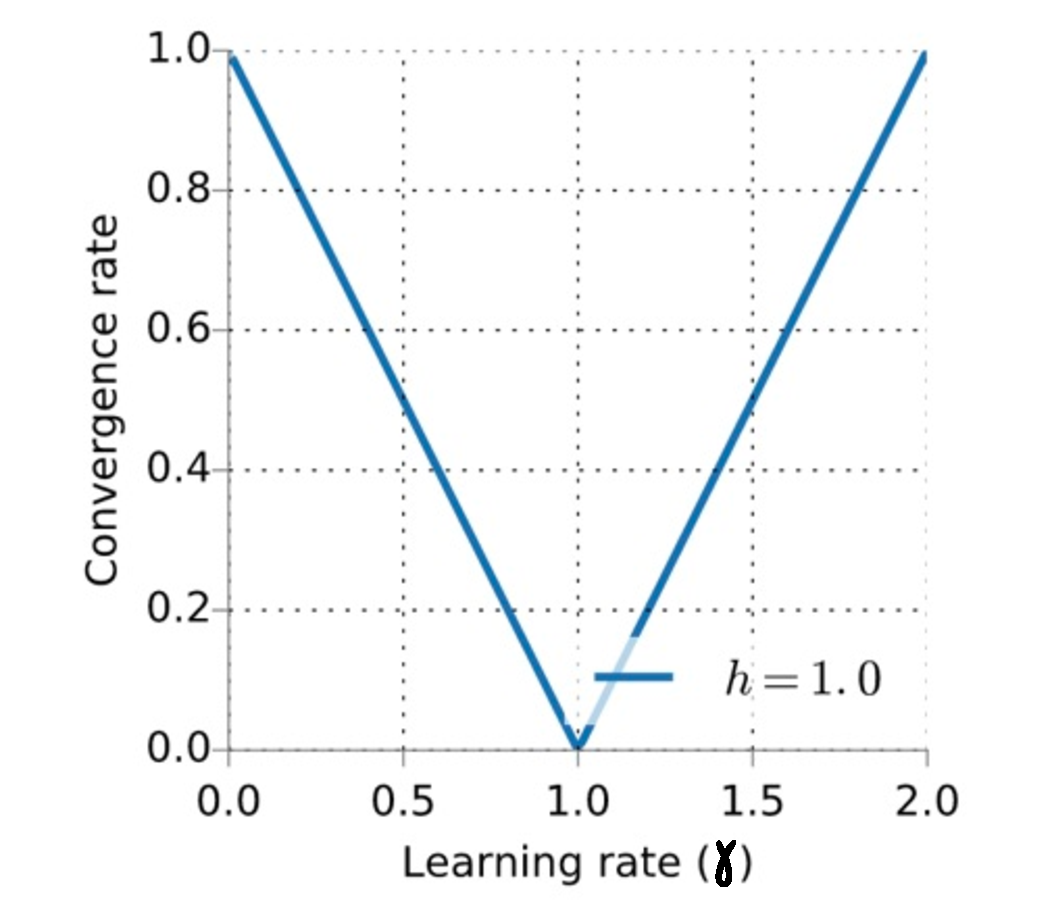
\includegraphics[height=2in]{GD_ro_vs_lr.pdf}}%
\qquad
\subfigure{%/
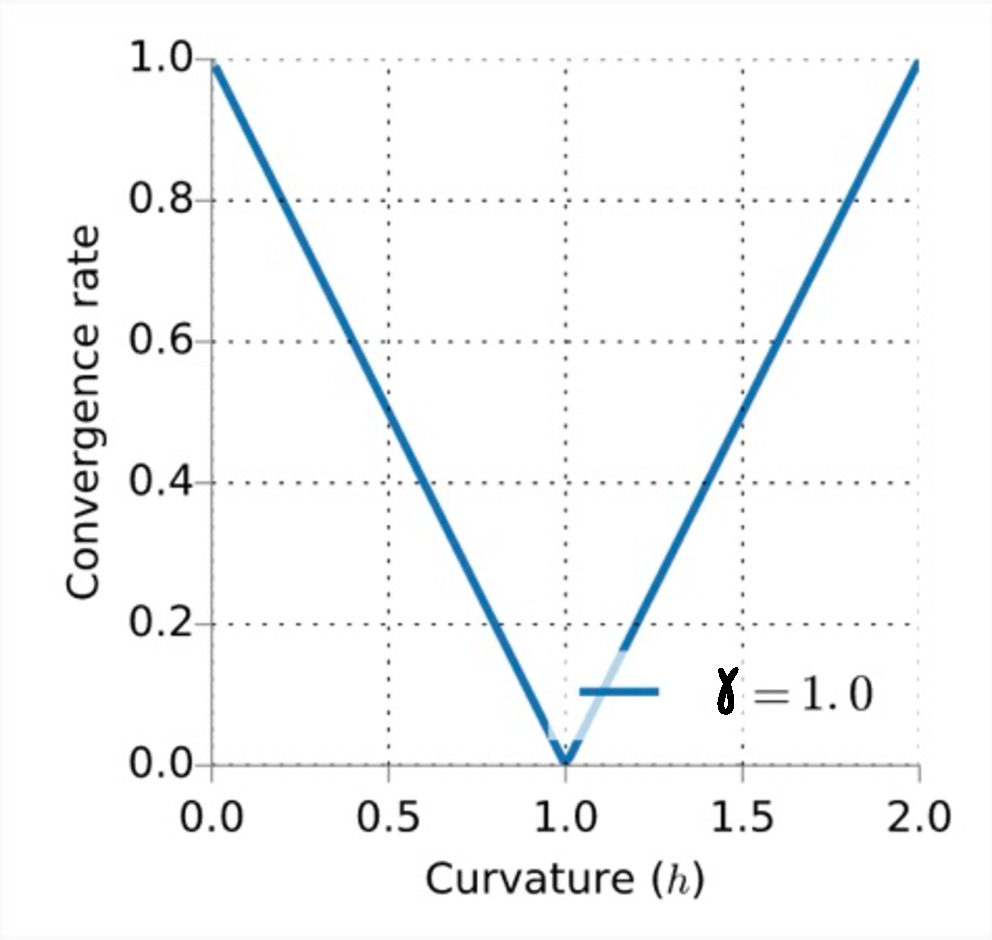
\includegraphics[height=2in]{GD_ro_vs_curv.pdf}}%
\caption{Convergence rate as a function of the learning rate (left plot) and curvature (right plot), for the function $\frac{h}{2}x^2$,~\cite{mitliagkas2019interesting}.}
\label{fig:convergence-plots}
\end{figure}

Moving on to a multivariate quadratic objective function, we assume without loss of generality that the Hessian $H$ is diagonal.
We can make this assumption because if $H$ is general non-diagonal, and symmetric by definition, we can always do a decomposition into $H = U\Lambda U^T$ and a change of basis to get a diagonal Hessian:
\begin{equation}
    f(x) = \frac{1}{2} x^T U \Lambda U^T x, \text{ with } w=U^T x \text{ giving } f(w) = \frac{1}{2} w^T \Lambda w
\end{equation}

Suppose then that we have the following quadratic:
\begin{equation}
f(x) = \frac{1}{2} x^T H x \quad \text{where } H = \begin{pmatrix} h_1&0&0\\0&h_2&0\\0&0&h_3\end{pmatrix}
\end{equation}
We can further decompose the vector dynamics into scalar dynamics dependent on eigendirections, where we denote with $i$ the component of the vector $x$ and the correspondent curvature in the Hessian $h$. 

\begin{align*}
	x_{t+1}(i) &= x_t(i) -\gamma h(i) x_t(i) \\
            &=(1 - \gamma h(i)) x_t(i) \\
            &=(1 - \gamma h(i))^t x_1(i)
\end{align*}

Taking the following concrete example, where 
\begin{equation}
H = \begin{pmatrix} 1&0&0\\0&2&0\\0&0&3\end{pmatrix}
\end{equation}
we observe that we get contrasting convergence rates for different directions that have distinct curvatures. The convergence rate thus decomposes into a sum where the largest convergence rate dominates - indicated by the lowest eigenvalue:
\begin{equation}
||x_t - x^*||^2 \leq c1 \rho_1^{2t} + c2 \rho_2^{2t} + c3 \rho_3^{2t}.
\end{equation}

Note the convergence rate for a given curvature will vary depending on the learning rate. In the left plot of Figure~\ref{fig:multivar_conv}, convergence rate continues to decrease with an increasing curvature and a learning of $\gamma = 0.25$. In the right plot of Figure~\ref{fig:multivar_conv}, convergence diverges with increasing curvature, for a learning rate of $\gamma=0.75$.

We can establish then that the goal is to find:
\begin{equation}
\min_\gamma \max \{\rho_1, \rho_2, \rho_3\}
\end{equation}

\begin{figure}[H]%
\centering
\subfigure{%
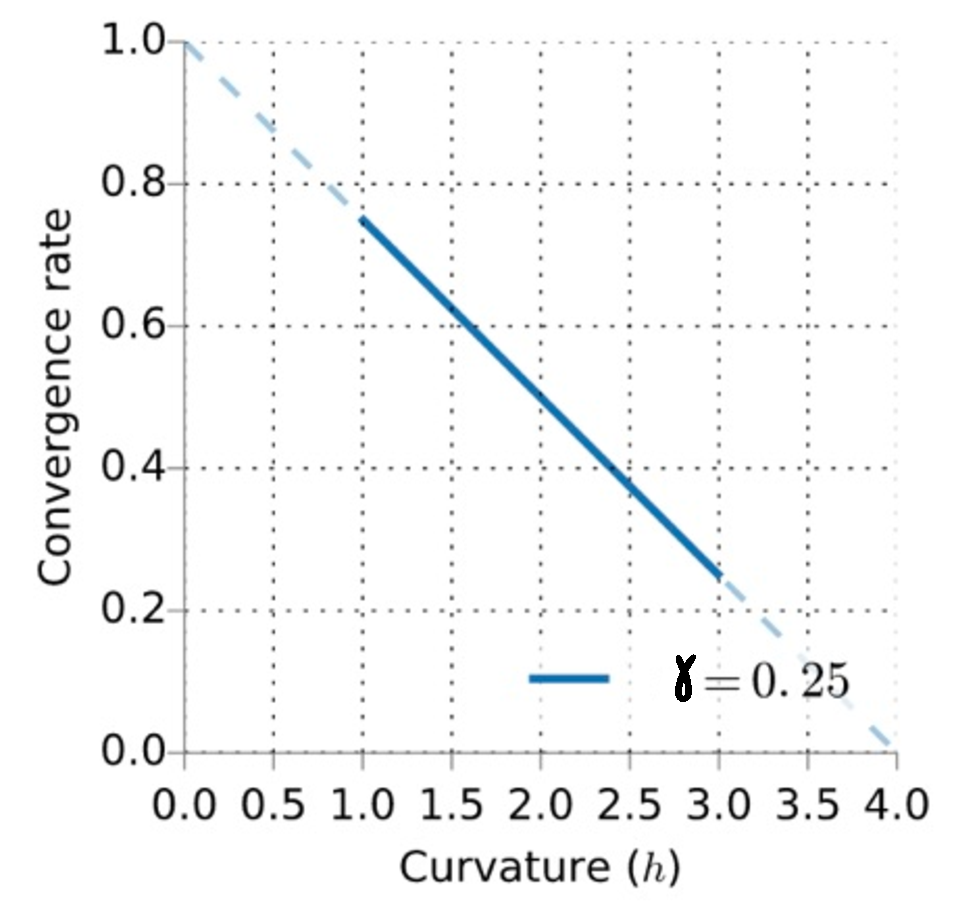
\includegraphics[height=2in]{multivar_GD_ro_vs_curv_alpha_0_25.pdf}}%
\qquad
\subfigure{%
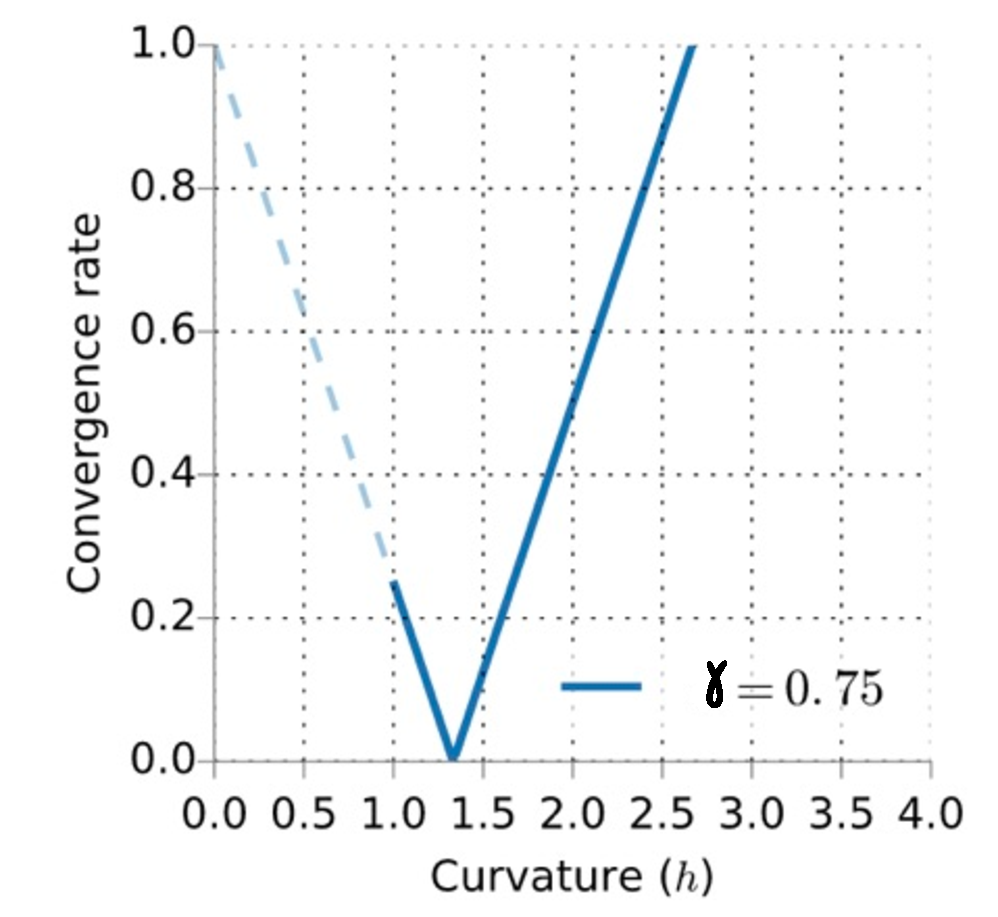
\includegraphics[height=2in]{multivar_GD_ro_vs_curv_alpha_0_75.pdf}}%
\caption{Convergence rate as a function of curvature. The left plot shows convergence with learning rate $\gamma = 0.25$, and $\gamma = 0.75$ for the right plot,~\cite{mitliagkas2019interesting}.}
\label{fig:multivar_conv}
\end{figure}

Figure~\ref{fig:optimal_alpha} shows that the optimal learning rate is that which balances the convergence rate between extreme curvatures. Setting the convergence rate to be equal for the smallest and largest eigenvalues, we can solve for the optimal step size and rate:
\begin{equation}
|1 - \gamma h_{\min}| = |1 - \gamma h_{\max}|
\end{equation}
\begin{equation}
\gamma^* = \frac{2}{h_{\min} + h_{\max}} = 0.5
\end{equation}

\begin{figure}[H]%
\centering
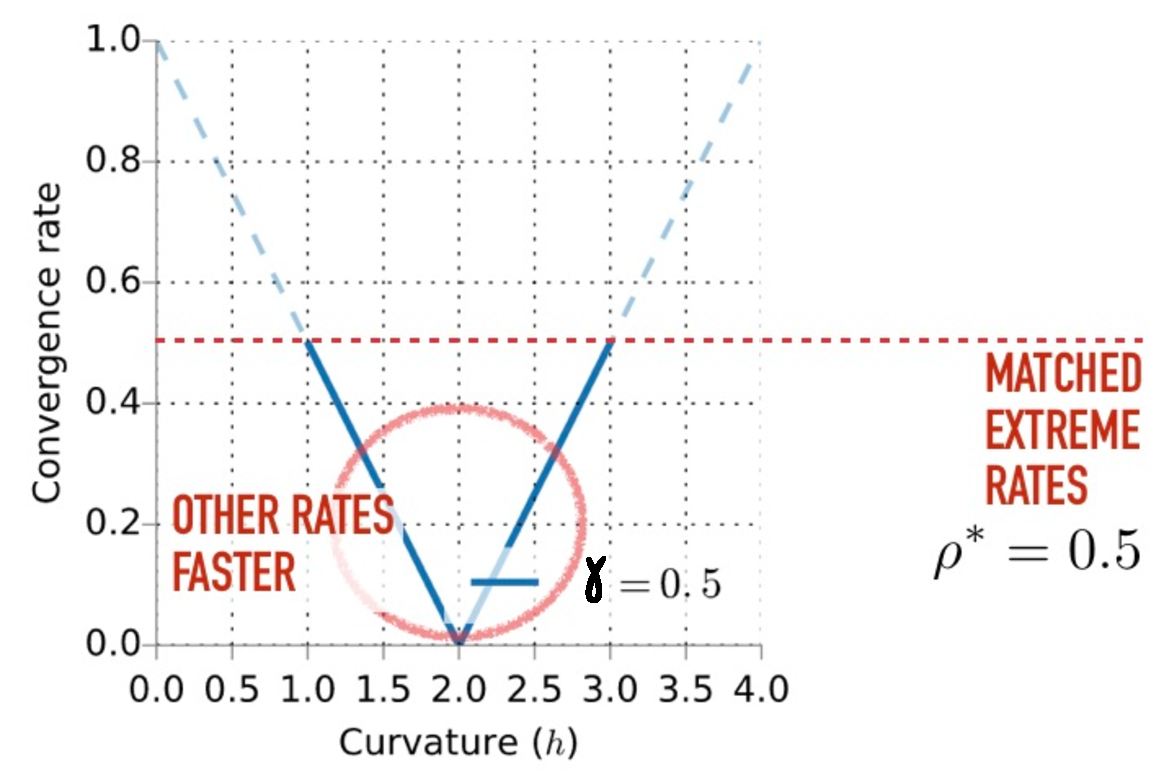
\includegraphics[height=2in]{GD_optimal_lr.pdf}
\caption{Convergence rate as a function of curvature given the optimal learning rate,~\cite{mitliagkas2019interesting}.}
\label{fig:optimal_alpha}
\end{figure}

It may seem strange that the dimension with highest curvature would converge at the same rate as the dimension with lowest curvature, as shown in Figure~\ref{fig:optimal_alpha}. The intuition is that the sequence of updates oscillates in the dimension with highest curvature, while in the other one convergence is very slow.

\section{Polyak's momentum}
Momentum gradient descent, or the heavy ball algorithm was first proposed in the 60s. It combines the current gradient with a history of the previous step to accelerate the convergence of the algorithm. For example, the images below show a  valley like landscape, where the algorithm wants to reach the optimal point. 

\begin{figure}[H]%
\centering
\subfigure{%
\label{fig:without_mom}%
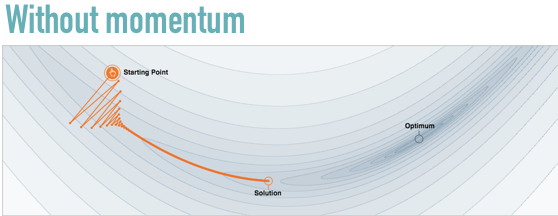
\includegraphics[height=1in]{without_momentum.png}}%
\qquad
\subfigure{%
\label{fig:with_mom}%
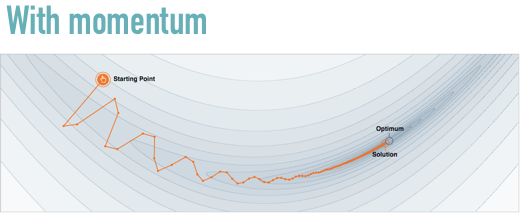
\includegraphics[height=1in]{with_momentum.png}}%
\caption{Without momentum, gradient descent oscillates, whereas with momentum, we find that it converges much closer to the optimal point in the same number of iterations,~\cite{goh2017why}.}
\end{figure}

Polyak's momentum, also known as the ``heavy ball method'', introduces a ``momentum'' term $\mu(x_t-x_{t-1})$, inspired by physics interpretations. If we imagine the current iterate as an object with mass, then our gradient descent update should be proportional to the previous step size. The full momentum update is:

\begin{equation}
x_{t+1} = x_t - \gamma \nabla f(x_t) + \mu(x_t-x_{t-1})
\end{equation}
where $\mu$ is a hyperparameter (typically $\mu \in [0,1]$, although not limited to it), which scales down the previous step. Adding this scaled previous step controls oscillation and in low curvatures causes acceleration along the same direction. The overall effect is that it allows the step size $\gamma$ to be larger and decreases the number of steps to convergence, which is illustrated in the change of convergence rate.
\\

Figure~\ref{fig:conv_momentum} illustrates how the convergence rate dynamics change in this case, i.e. we achieve the same rate of convergence for all curvature - a property unique to Polyak's momentum.

\begin{figure}[H]%
\centering%
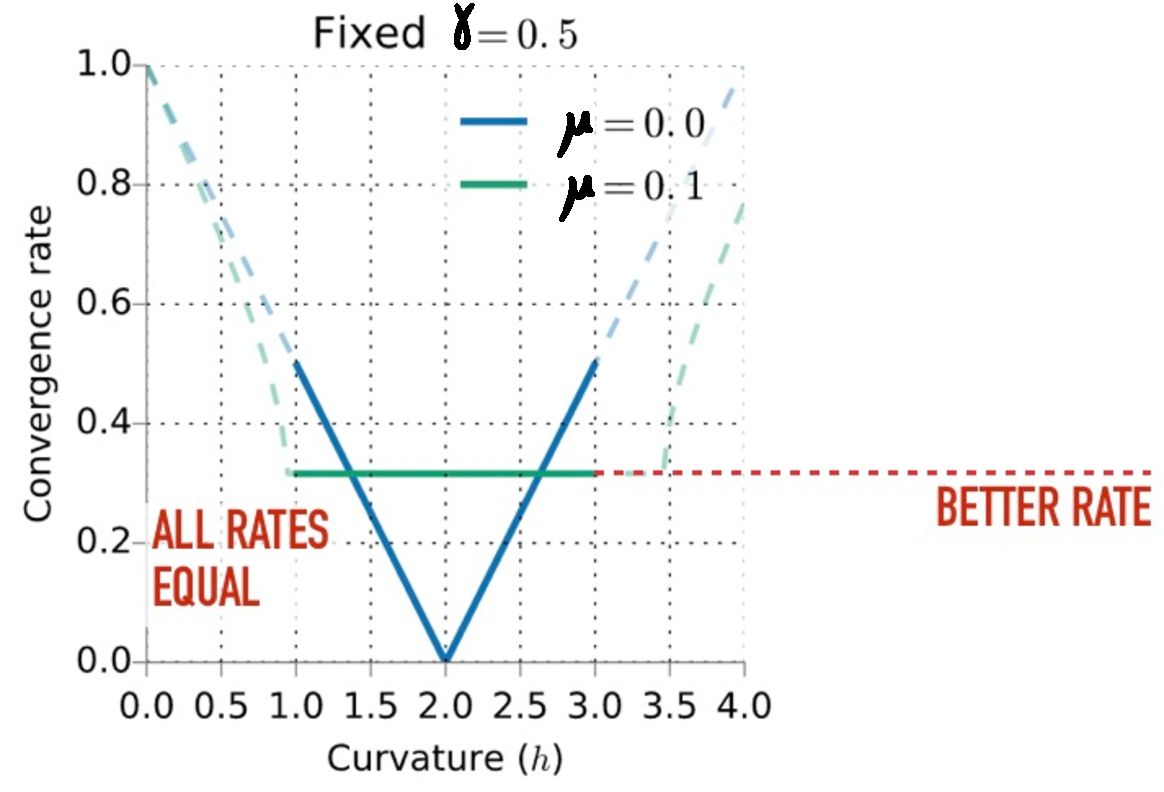
\includegraphics[height=2in]{polyak.pdf}
\caption{Convergence rate as a function of curvature. The blue curve is standard gradient descent without momentum, whereas the green curve includes momentum with $\mu = 0.1$,~\cite{mitliagkas2019interesting}.}
\label{fig:conv_momentum}
\end{figure}

\subsection{Convergence rate of Polyak's Momentum for a quadratic loss}

Going back to our previous scalar quadratic objective:
\begin{equation}
	f(x) = \frac{h}{2} x^2
\end{equation}

Let's write the momentum update rule for this function and do some simple algebraic manipulations to obtain a more convenient form:
\begin{align*}
    x_{t+1} &= x_t - \gamma \nabla f(x_t) + \mu(x_t - x_{t-1}) \\
    &= x_t - \gamma h x_t + \mu(x_t - x_{t-1}) \\
    &= (1 + \mu - \gamma h)x_t - \mu x_{t-1}
\end{align*}
We can further write the above equation as a linear system:
\begin{equation}
	\begin{bmatrix}x_{t+1}\\x_{t}\end{bmatrix} = \begin{bmatrix}1-\gamma h + \mu &-\mu \\1&0\end{bmatrix}\begin{bmatrix}x_{t}\\x_{t-1}\end{bmatrix} 
\end{equation}
Note the recursive property of the above. By denoting the linear operator with $A$, we can recurse $A$ for $t$ steps and express $x_{t+1}, x_t$ as a function of starting values $x_1, x_0$:
\begin{equation}
\begin{bmatrix}x_{t+1}\\x_{t}\end{bmatrix} = A^t\begin{bmatrix} x_{1}\\x_{0}\end{bmatrix} 
\end{equation}


Consider comparing our iterated $x_t$ with optimal $x^*$:
%\begin{equation}
%\begin{bmatrix}x_{t+1} - x^*\\x_{t} - x^*\end{bmatrix} = A^t\begin{bmatrix} x_{1} - x^*\\x_{0} - x^*\end{bmatrix} 
%\end{equation}

%Taking the norm:
%
%\begin{equation}
%\left\lVert  \begin{bmatrix}x_{t+1} - x^*\\x_{t} - x^*\end{bmatrix}  \right\rVert_2  = \left\lVert A^{t}  \begin{bmatrix}x_{1}- x^*\\x_{0} - x^*\end{bmatrix}  \right\rVert_2 \leq
%\left\lVert A^{t}  \right\rVert_2 \left\lVert \begin{bmatrix}x_{1}- x^*\\x_{0} - x^*\end{bmatrix}  \right\rVert_2 
%\end{equation}
%
%there must exist a matrix norm such that: 
%
%\begin{equation}
%\left\lVert A^{t} \right\rVert \leq (\rho(A) + \epsilon)^{t}
%\end{equation}
%
%with $\rho(A) = \max{\{|\lambda_1|,|\lambda_2|\}}$ (spectral radius, or the max of the two eigenvalue magnitudes). Therefore,   
%\begin{equation}
%\left\lVert \begin{bmatrix}x_{t+1} - x^*\\x_{t} - x^*\end{bmatrix}  \right\rVert_2 \leq (\rho(A) + \epsilon)^{t} \left\lVert \begin{bmatrix}x_{1} - x^*\\x_{0} - x^*\end{bmatrix}  \right\rVert_2 
%\end{equation}
%
%
%Noting that asymptotically the spectral radius of $A$ gives the convergence rate:
%\begin{equation}
%\left\lVert\begin{bmatrix}x_{t+1} - x^*\\x_{t} - x^*\end{bmatrix} \right\rVert_2=O(\rho (A)^t),
%\end{equation}

\begin{align}
\label{eq:gdwqobiwqd}
\begin{bmatrix}x_{t+1} - x^*\\x_{t} - x^*\end{bmatrix}  &=  A^{t}  \begin{bmatrix}x_{1}- x^*\\x_{0} - x^*\end{bmatrix}, \nonumber \\
\left\lVert  \begin{bmatrix}x_{t+1} - x^*\\x_{t} - x^*\end{bmatrix}  \right\rVert_2 &= \left\lVert A^{t}  \begin{bmatrix}x_{1}- x^*\\x_{0} - x^*\end{bmatrix}  \right\rVert_2, \nonumber \\
					&\leq \left\lVert A^{t}  \right\rVert_2 \left\lVert \begin{bmatrix}x_{1}- x^*\\x_{0} - x^*\end{bmatrix}  \right\rVert_2.
\end{align}
\pagebreak
\par One could be tempted to note that:
\begin{align}
    \|A^t\|_2 &\le\|A\|_2^t, && \text{(submultiplocativity of norms, see \cite{simon2012spectralradius}, p. 4)}, \nonumber \\
            &=\sqrt{\rho(A^TA)}^t, && \text{(Theorem \ref{th_eq_sprad_m2nrm}, Appendix \ref{sec:matrix_norm_and_spectral_radius})}, \nonumber
\end{align}
where $\rho(\cdot)$ denotes the spectral radius.
\\
\par Unfortunately, this result produces a diverging upper bound if combined into (16), since $\sqrt{\rho(A^TA)}>1$ (we do not demonstrate this inequality here).
\\
\par Thankfully, Theorem \ref{th_mnrm_ubound} (Appendix \ref{sec:matrix_norm_and_spectral_radius}) provides the means for obtaining the converging bound we seek.
\\
\par This Theorem, when applied to matrix $A$ and for a chosen constant $\epsilon > 0$ (more on this later),  provides that a norm, denoted below $||| \cdot |||$, exists that verifies:
\begin{align}
	\label{eq:wdojqwqwd}
	|||A||| \le \rho(A) + \epsilon.
\end{align}
\\
\par Furthermore, following an argument in \cite{simon2012spectralradius}, page 7, the equivalence of the norms provides that there exists a constant $\text{C}>0$ for which:
\begin{align}
	\| M \|_2 &\le \text{C} ||| M |||, \qquad \forall \text{ }M \in \mathds{C}^{n\times n}. \nonumber
\end{align}
\par Hence
\begin{align}
	\| A^t \|_2	&\le \text{C} ||| A^t |||, \nonumber \\
			&\le \text{C} ||| A |||^t, \qquad \text{(submultiplicativity of norms, see \cite{simon2012spectralradius}, p. 4)}.\nonumber
\end{align}
\par Use of (\ref{eq:wdojqwqwd}) now yields
\begin{align}
	\label{eq:pefnponweffe}
	\| A^t \|_2 &\le \text{C} ||| A |||^t \le \text{C} \left( \rho\left(A\right) + \epsilon \right)^t, \nonumber
\end{align}
which by combining back into (\ref{eq:gdwqobiwqd}) yields
\begin{align}
\left\lVert  \begin{bmatrix}x_{t+1} - x^*\\x_{t} - x^*\end{bmatrix}  \right\rVert_2 &\leq \text{C} \left( \rho\left(A\right) + \epsilon \right)^t  \left\lVert \begin{bmatrix}x_{1}- x^*\\x_{0} - x^*\end{bmatrix}  \right\rVert_2, \nonumber\\
\left\lVert  \begin{bmatrix}x_{t+1} - x^*\\x_{t} - x^*\end{bmatrix}  \right\rVert_2 &= \mathcal{O} \left( \rho\left(A\right)^t + \epsilon^t \right), \qquad \epsilon >0. \nonumber
\end{align}

Since we can set $\epsilon \ll \rho\left( A \right)$, in practice we discard the term in $\epsilon$ for conciseness (although this is not absolutely rigorous) and we obtain the following upper bound on the convergence rate:
\begin{align}
\left\lVert  \begin{bmatrix}x_{t+1} - x^*\\x_{t} - x^*\end{bmatrix}  \right\rVert_2 &= \mathcal{O}  \left( \rho\left(A\right)^t \right). \nonumber
\end{align}

\subsection{Robust region and optimal step size} % <--- Added this

If we write down the algebraic form of the determinant:
\begin{equation}
det(A) = \lambda_1 \lambda_2 = \mu
\end{equation}
we can observe that it is not dependent on $\gamma$ and this gives an intuitive reason for the flatness of the convergence rate.
\\

We can now do an analysis of the spectral radius of the momentum operator $A$:
\begin{equation}
A=\begin{bmatrix}1-\gamma h + \mu &-\mu \\1&0\end{bmatrix}
\end{equation}

Figure~\ref{fig:robust_region} shows the two distinct dynamics region induced by the discriminant:
\begin{equation}
\Delta = tr(A)^2 - 4 det(A)
\end{equation}
We can observe that when $\Delta > 0$ we get two real eigenvalues and when $\Delta < 0$ we have two complex conjugate eigenvalues $\frac{(1-\sqrt{\mu})^2}{h} \leq \gamma \leq \frac{(1+\sqrt{\mu})^2}{h}$. We can visualize this process in the figure \ref{fig:robust_region}, where we can see that the two eigenvalues split at some point and become conjugate of each other and as such we enter a robust region where the rate of convergence is $\rho(A) = \sqrt{\mu}$. Also note that the width of the robust region is given by $\mu$.

We can demonstrate this by explicitly computing the eigenvalues of our matrix:
\begin{align}
    \lambda_1 &= \frac{1}{2}\left(1-\gamma h + \mu + \sqrt{(-\gamma h + \mu + 1)^2 - 4 \mu} \right) \\
    \lambda_2 &= \frac{1}{2}\left(1-\gamma h + \mu - \sqrt{(-\gamma h + \mu + 1)^2 - 4 \mu} \right)
\end{align}

When $(-\gamma h + \mu + 1)^2 - 4 \mu < 0$, then the roots are complex conjugates, which implies the absolute values of the eigenvalues are identical. Therefore: 

\begin{equation}
    \vert \lambda_1 \vert = \vert \lambda_2 \vert = \sqrt{(1-\gamma h + \mu)^2 + \vert (-\gamma h + \mu + 1)^2 - 4\mu \vert } = \sqrt{\mu}
\end{equation}

Which implies the converge rate is the same and solely dependent on $\mu$. This leads to the following lemma.

\begin{lemma} [Robust Region]
For some choice of $\gamma$, the absolute eigenvalues are identical and
\[
\rho(A) = \sqrt{\mu}
\]

holds for a ``robust region'', that is to say the convergence rate is constant for the range of $\gamma$ where the discriminant of the momentum operator $A$ is less than 0.
\end{lemma}

\begin{figure}[H]%
\centering
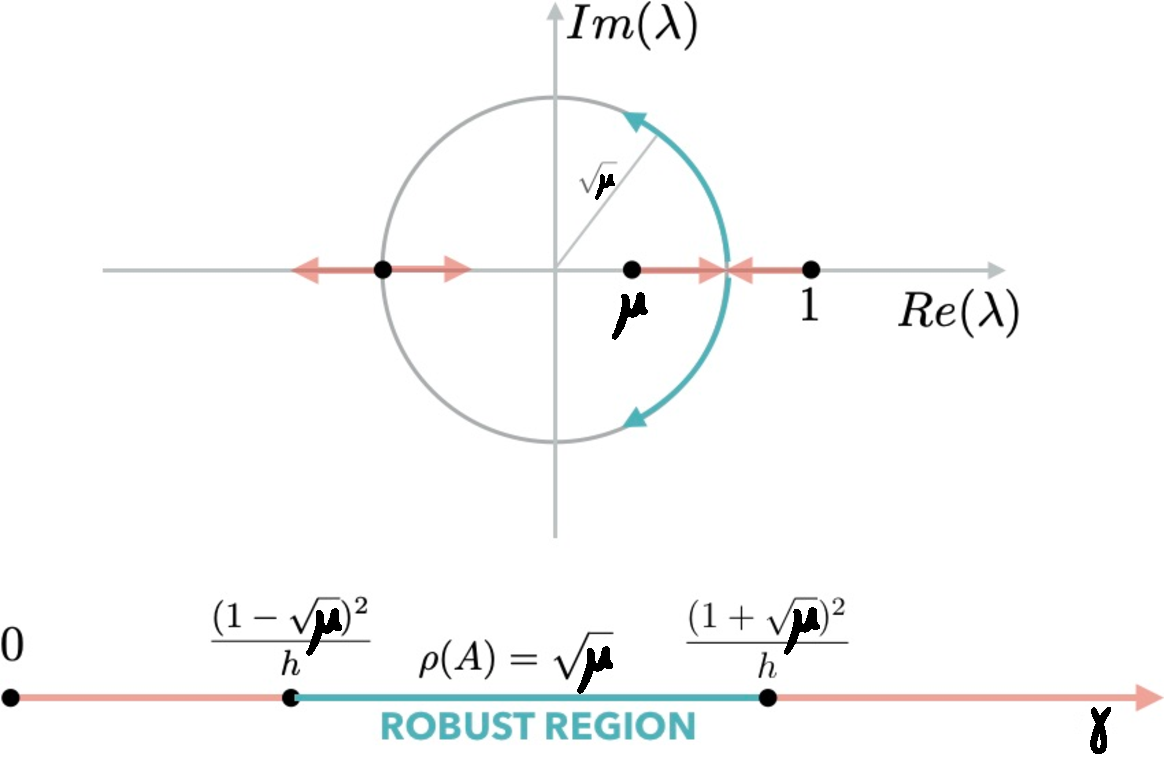
\includegraphics[height=2in]{discriminator_analysis.pdf}%
\caption{Real and imaginary eigenvalues of the momentum operator A with varying learning rates,~\cite{mitliagkas2019interesting}.}
\label{fig:robust_region}%
\end{figure}


The images below depict the rate  of convergence with respect to the curvature and the step size. We can note that larger values of $\mu$ give larger widths for the robust region, but also larger rate of convergence.
\begin{figure}[H]%
\centering
\subfigure{%
\label{fig:robust_alpha}%
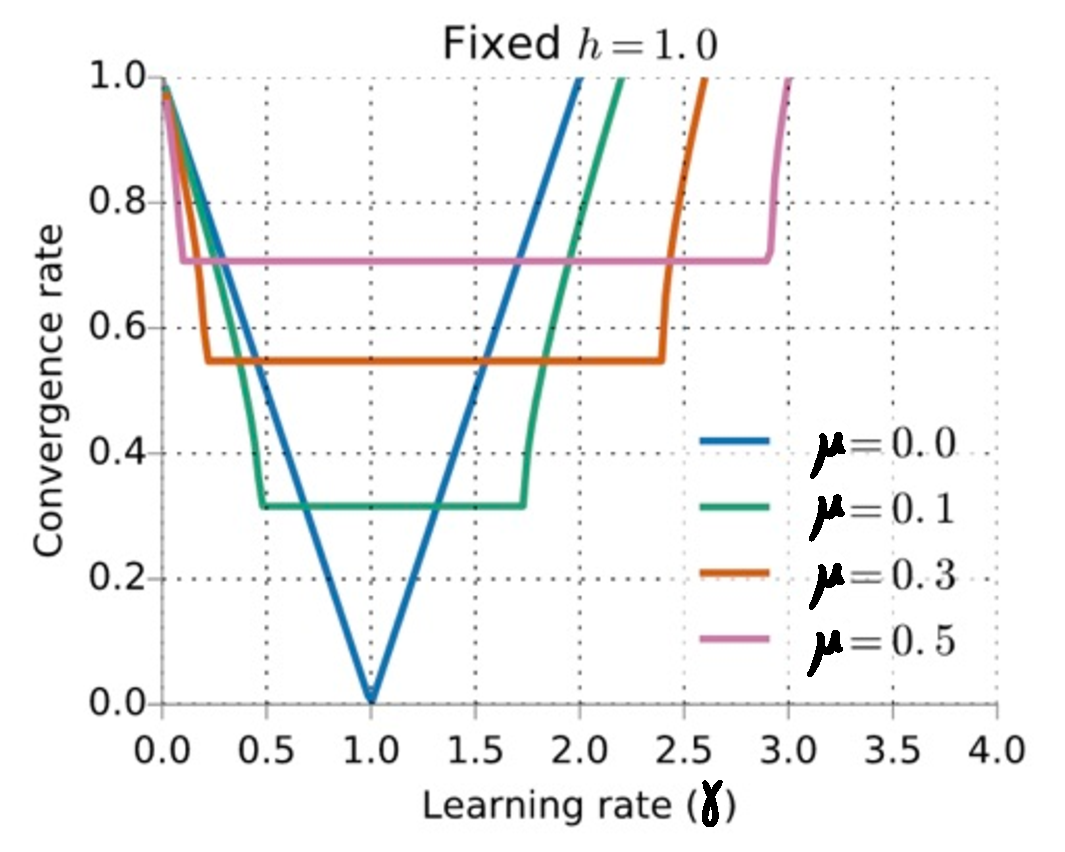
\includegraphics[height=2in]{polyak_plot1.pdf}}%
\qquad
\subfigure{%
\label{fig:robust_curvature}%
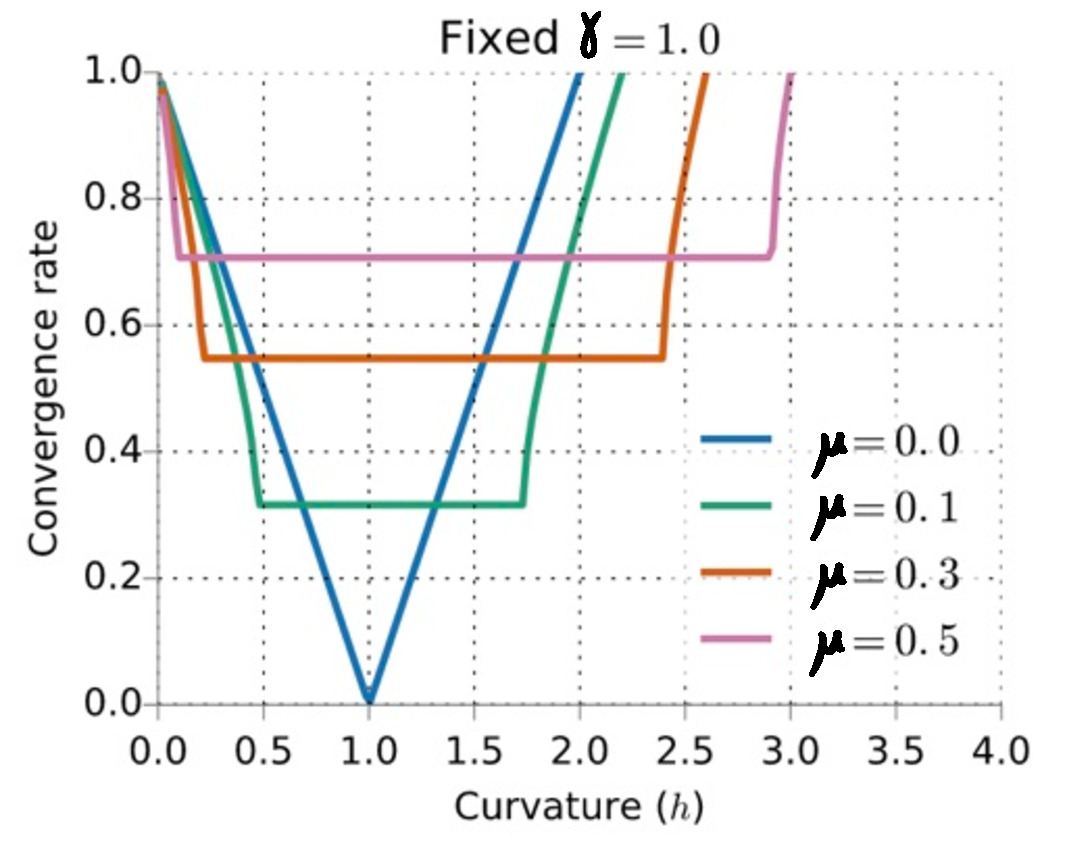
\includegraphics[height=2in]{polyak_plot2.pdf}}%
\caption{Convergence rates displaying robust regions as a function of learning rate and curvature for various momentum sizes,~\cite{mitliagkas2019interesting}.}
\end{figure}



Note that as we increase the width of the robust regions for the extreme curvatures, the point where the two regions meet corresponds to the optimal step size. Consequently, this leads to the following optimal step size lemma.

\begin{lemma}[Optimal $\gamma, \mu$]
The optimal step size $\gamma$ is given by:
  
\begin{equation}
\gamma^* = \frac{(1 + \sqrt{\mu})^2}{h_{\max}} = \frac{(1 - \sqrt{\mu})^2}{h_{\min}},
\end{equation}
from which the value of the optimal rate of convergence $\rho$ can be derived as:
\begin{equation}
\rho^* = \sqrt{\mu^*} = \frac{\sqrt{\kappa} - 1}{\sqrt{\kappa} + 1} \underset{\text{for\ large\ k}}{\approx \exp(-\frac{C}{\sqrt{\kappa}})},
\end{equation}
where $\kappa$ denotes the condition number $\kappa=\frac{h_{\max}}{h_{\min}}$, and $\mu$ is the momentum coefficient
\end{lemma}

\pagebreak

\appendix
%\input{matrix_norm_and_spectral_radius.tex}
\section{Spectral radius $\rho(\cdot)$ and operator norm $\| \cdot \|$}
\label{sec:matrix_norm_and_spectral_radius}
\subsection*{Definitions}
\begin{defn}[Operator Norm, \cite{simon2012spectralradius}, Def. 8]
If $\| \cdot \|$ is a vector norm on $\mathds{C}^n$, then the induced norm $\| \cdot \|$ on $\mathds{C}^{n\times n}$ defined by
\[
	\|A\| \triangleq \max_{\|x\|=1}\|Ax\|
\]
is a matrix norm on $\mathds{C}^{n\times n}$. 
\end{defn} 
\par Note that in that the notation $\| \cdot \|$ is overloaded in the above definition: it designates the vector norm for a vector argument, and an operator norm for a matrix argument. In particular, we note $\| \cdot \|_q$ the operator norm induced by the vector norm $\| \cdot \|_q$, e.g.:
\begin{align}
	\|A\|_1 &\triangleq \max_{\|x\|_1=1}\|Ax\|_1, \nonumber \\
	\|A\|_2 &\triangleq \max_{\|x\|_2=1}\|Ax\|_2. \nonumber
\end{align}

\begin{defn}[Spectral Radius, \cite{simon2012spectralradius}, Sec. 3]
The spectral radius of a matrix $M\in \mathds{C}^{n\times n}$ is given by:
\[
	\rho(A) \triangleq \max \left\{ |\lambda|, \lambda \text{ eigenvalue of }A\right\}
\]
\end{defn}

\subsection*{Equality relations (for $\| \cdot \|_2$ only)}
Equality relations exist between the spectral radius and the matrix 2-norm specifically. These are cited here for completeness as they are not used in the development of the convergence rate bound.
\begin{thm}[\cite{simon2012spectralradius}, Proposition 9]
\label{th_eq_sprad_m2nrm}
\[
	\|A\|_2 = \sqrt{\rho(A^*A)}, \qquad \forall \text{ } A \in \mathds{C}^{n\times n}. 
\]
\end{thm}
\par This relation simplifies further if the matrix is hermitian symmetric.
\begin{thm}[\cite{simon2012spectralradius}, page 5]
\[
	\|A\|_2 = \rho(A), \qquad \forall \text{ } A \in \mathds{C}^{n\times n} \text{ and  hermitian, i.e. for which } A^*=A.
\]
\end{thm}

\subsection*{Inequality relations}
\par The following inequalities hold more generally. Note that the first one is cited for completeness: it is not used in the development of the convergence rate bound. However the second one is.
\begin{thm}[Lower bound on operator norm, \cite{simon2012spectralradius}, Lemma 10]
\[
	\rho(A) \le \|A\|, \qquad \forall \text{ } A \in \mathds{C}^{n\times n}.
\]
\end{thm}

\begin{thm}[Upper bound on operator norm, \cite{simon2012spectralradius}, Lemma 11] Given $A\in \mathds{C}^{n\times n}$ and $\epsilon>0$, there exists a norm $\|\cdot \|$ such that
\label{th_mnrm_ubound}
\[
	\|A\| \le \rho(A) + \epsilon.
\]
\end{thm}

\pagebreak
\bibliography{Refs/lec5.bib}
\bibliographystyle{abbrvnat}
%----------------------------------------
\end{document}
https://v2.overleaf.com/project/5c4e654fc5a65f316fbc4ec6